\documentclass[12pt,a4paper]{article}
\usepackage[utf8]{inputenc}
\usepackage{graphicx}
\usepackage{geometry}
\usepackage{enumitem}
\usepackage{titlesec}
\usepackage{hyperref}

\geometry{margin=2.5cm}

\title{Student Loyalty Analysis}
\date{}

\begin{document}

\maketitle

\section*{1. Loyalty Distribution}
As shown in Figure~\ref{fig:loyalty-distribution}, the majority of students (244 individuals) registered for only one course, highlighting a strong skew toward one-time participation. In contrast, only 35 students enrolled in two courses and just 13 students participated in three courses. This means over 83\% of students are non-loyal (single-course attendees).

This suggests that while the academy attracts a large number of students, retention and repeat engagement are limited, and there may be untapped potential in encouraging re-enrolment.

\begin{figure}[h!]
    \centering
    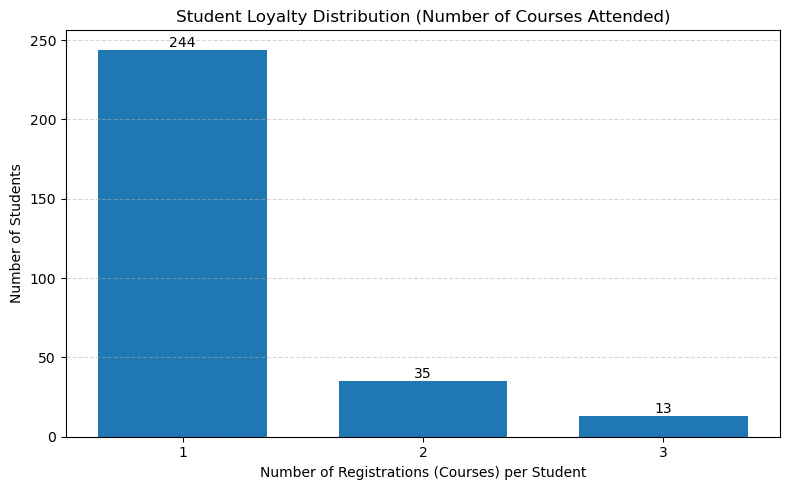
\includegraphics[width=0.9\textwidth]{Student Loyalty Distribution (Number of Courses Attended).png}
    \caption{Student Loyalty Distribution (Number of Courses Attended)}
    \label{fig:loyalty-distribution}
\end{figure}

\section*{2. Income Contribution by Loyalty Segment}
Figure~\ref{fig:loyalty-income} shows that despite their smaller number, loyal students (those who registered for more than one course) contributed approximately 25.7\% of total income, while non-loyal students were responsible for 74.3\%.

Although loyal students are a minority, their higher lifetime value is evident. This finding underscores the importance of developing targeted strategies (e.g., loyalty programs, follow-up offers) to increase repeat registrations.

\begin{figure}[h!]
    \centering
    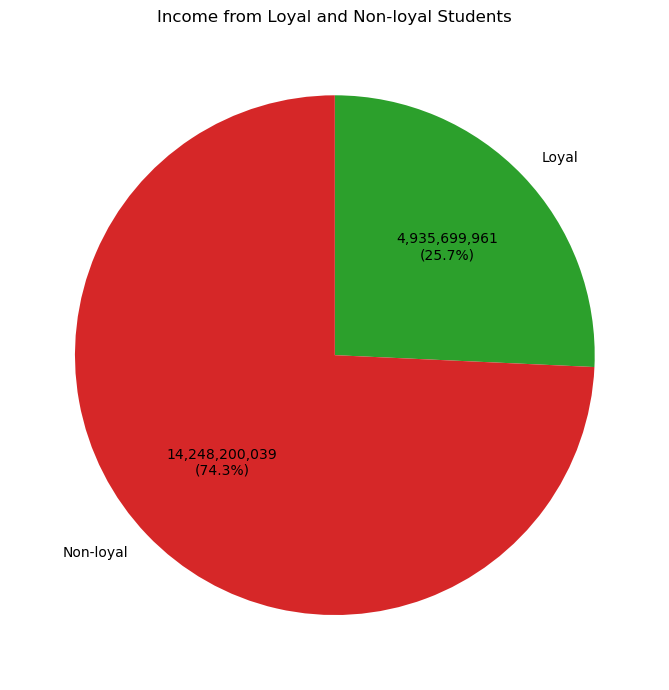
\includegraphics[width=0.8\textwidth]{Income from Loyal and Non-loyal Students (Pie Chart).png}
    \caption{Income from Loyal and Non-loyal Students}
    \label{fig:loyalty-income}
\end{figure}

\section*{Summary}
\begin{itemize}
    \item Most students register once and do not return.
    \item Loyal students generate disproportionately higher income.
    \item Improving student retention could significantly enhance revenue without requiring a proportional increase in new student acquisition.
\end{itemize}

\end{document}